\documentclass[openany]{book} % Use 'book' for double-sided printing
\usepackage{babel}
%\usepackage[portuguese]{babel}

% Define trim size and bleed
\newlength{\trimwidth}
\newlength{\trimheight}
\setlength{\trimwidth}{6.69in}
\setlength{\trimheight}{9.61in}
\newlength{\bleed}
\setlength{\bleed}{0.125in}
\newlength{\textmargin}
\setlength{\textmargin}{0.5in}
\newlength{\topbottommargin}
\setlength{\topbottommargin}{1in}
\newlength{\innermargin}
\setlength{\innermargin}{0.75in}

% Calculate total paper dimensions
\newlength{\mypaperwidth}
\newlength{\mypaperheight}
\setlength{\mypaperwidth}{\trimwidth} % Base width
\addtolength{\mypaperwidth}{\bleed}   % Add outer bleed
\setlength{\mypaperheight}{\trimheight}
\addtolength{\mypaperheight}{2\bleed} % Add top and bottom bleeds
\usepackage[paperwidth=\mypaperwidth,paperheight=\mypaperheight]{geometry} % Temporary base paper size for compilation

% Set up geometry with asymmetric margins for odd/even pages
\geometry{
  left=\textmargin,
  right=\textmargin,
  inner=\innermargin,
  top=\topbottommargin,
  bottom=\topbottommargin,
}

\usepackage{amsmath}
\usepackage{amsfonts}
\usepackage{tikz}
\usetikzlibrary{arrows.meta, decorations.pathmorphing}

\usepackage{pdfpages}
\usepackage{fancyhdr} % For custom headers/footers (often used in books)
\usepackage{graphicx}
\usepackage{eso-pic}

% --- Custom Header/Footer Setup (Example using fancyhdr) ---
% You might already have this set up in your book's class or style file
\pagestyle{fancy}
\fancyhf{} % Clear all header and footer fields
\fancyhead[LE,RO]{\thepage} % Page number on left even, right odd
%\fancyhead[LO]{\rightmark} % Chapter title on left odd
%\fancyhead[RE]{\leftmark}  % Section title on right even (if using sections)
%\fancyfoot[C]{\textit{Your Author Name}} % Author in the center footer

\renewcommand{\headrulewidth}{0pt} % NO line under header
\renewcommand{\footrulewidth}{0pt} % NO line above footer
% -----------------------------------------------------------


\usepackage{fontspec}
%\setmainfont{Comic Sans MS}
%\setmainfont{Comic Neue}
\setmainfont{Patrick Hand}
%\setmainfont[Ligatures=TeX]{Segoe Print}

\usepackage{hyperref}
\hypersetup{
    colorlinks,
    citecolor=black,
    filecolor=black,
    linkcolor=black,
    urlcolor=black
}

\title{The Grand Hotel Infinita}
\author{Leonardo Araújo}
\date{} 

\begin{document}
\pagenumbering{gobble}
\thispagestyle{empty}
\includepdf[pages=-]{cover.en.pdf}

%\thispagestyle{empty} % No page number on this page
%\newpage

\clearpage
\thispagestyle{empty} % No page number on this page
\mbox{}
\clearpage

%\frontmatter
\pagenumbering{arabic} % start numbering from here
\setcounter{page}{1}
\maketitle
\thispagestyle{empty}

\thispagestyle{empty} % No page number on this page

\vspace*{\fill} % Push content to the bottom

\begin{center}
    \textbf{\huge The Grand Hotel Infinita} % Added the main title

    %\vspace{0.5cm} % Space between main title and copyright info
    \large Copyright Information \textcopyright{} 2025 % Added copyright symbol and year
\end{center}

\vspace{1cm}

\begin{flushleft}
    \emph{Author:} Leonardo Araújo
\end{flushleft}

\vspace{0.5cm}

\begin{flushleft}
    \emph{License:} CC BY-NC-SA

    %\includegraphics[width=2cm]{cc-by-nc-sa.pdf}

    This work is licensed under the \href{https://creativecommons.org/licenses/by-nc-sa/4.0/}{Creative Commons Attribution-NonCommercial-ShareAlike 4.0 International License}.

    To view a copy of this license, visit \url{https://creativecommons.org/licenses/by-nc-sa/4.0/}.
\end{flushleft}

\vspace{0.5cm}

\begin{flushleft}
    \emph{Image Attributions:}

    \begin{itemize}
        \item Some images were created by the author, Leonardo Araújo.
        \item Some images were sourced from public domain or similarly licensed sources.
        \item Some images were generated using Artificial Intelligence (AI) tools.
    \end{itemize}
\end{flushleft}

\vspace*{\fill} % Push content to the top
\begin{center}
\includegraphics[width=2cm]{cc-by-nc-sa.pdf}
\end{center}

\newpage 


\Large
\tableofcontents % Table of contents

\clearpage
\includepdf[pages={1},
            pagecommand={\thispagestyle{fancy}}, % Apply your custom 'fancy' style
            fitpaper=true,
            noautoscale
           ]{infinity.pdf}
\clearpage 
\chapter*{Preface} % -- Embrace the journey of knowledge}
Have you ever wondered how big infinity is, or if one infinity could be bigger than another? Can a paradoxical, impossible problem have a perfectly logical solution? Mathematics, with its numbers, rules, and equations, might seem abstract, but it's actually an incredible tool that lets us explore worlds that only exist in our imagination.

In this story, you'll dive into the world of the Grand Hotel Infinita. It's a place where numbers guide the way, and infinity becomes a puzzle. Join a clever girl and her loyal four-legged friend to solve a mystery that seems impossible. Get ready to embark on a fantastic adventure where the impossible and mathematics unite, with a dash of humor, to solve a hairy problem!


%\mainmatter

\clearpage
\includepdf[pages={1},
            pagecommand={\thispagestyle{fancy}}, % Apply your custom 'fancy' style
            fitpaper=true,
            noautoscale
           ]{lobby.pdf}
\clearpage
\chapter{The Paradox and the Disappearing}
Nestled in the bustling heart of a glamorous city, a place where the world's most discerning travelers come to rest and recharge, stands a hotel that's both a destination and a time capsule: the Grand Hotel Infinita. It was an old, magnificent building, infinitely tall and wide, where history and luxury met. It was a place where every guest could escape the demands of the modern world and refill their energies in an environment of timeless elegance. Due to its size and age, the hotel had no passenger elevators, just an infinite number of stairs connecting all floors. To provide greater convenience, the hotel had recently installed a small, rattling freight elevator connected to every room. Guests could call the front desk to request snacks, drinks, or fresh towels, and their request would be delivered through the freight elevator.

The lobby, with its soaring ceilings, featured a sweeping marble staircase that seemed to climb forever. A massive chandelier cast a warm, golden light, creating a charming atmosphere. The front desk was a masterpiece of carved mahogany, manned by staff in impeccably tailored uniforms. At the desk sat Henrietta, a kind-hearted hippopotamus. Her assistant, Bernard, a diligent bellrat, stood by with polished luggage carts, awaiting the next guest. They were the hotel's only two staff members. With an infinite number of rooms to keep in order, they had to deal with an endless stream of guests arriving and leaving at all hours. It was a duty they fulfilled exquisitely, thanks to their superb organization and commitment to harmony.

\clearpage
\includepdf[pages={1},
            pagecommand={\thispagestyle{fancy}}, % Apply your custom 'fancy' style
            fitpaper=true,
            noautoscale
           ]{walrus.pdf}

On the night before the holiday, a distinguished walrus smoking a pipe was the last guest to arrive. He looked terribly tired as he walked in. Henrietta, always affectionately welcoming new guests, greeted him with a wide smile.

``It's a pleasure to welcome you to the Grand Hotel Infinita,'' she said. ``A place where the longing quest is left behind, where you may rest and ease your weary mind.'' 
%``A place where the longing quest is left behind, where you may rest and leave the whirlpool of wild dreams behind.''

``Oh, that's all I need,'' the walrus replied with a sigh of relief.

``Our hotel is quite full today, but you're in luck, Mr. Walrus! The first room on the first floor just became vacant!'' Henrietta exclaimed. ``Our agile Bernard will help you to your room instantly.''

Bernard led him to his room where he enjoyed a wonderfully restful night.

\vspace{4em}
The next morning was the start of an extended national holiday, the first after a long winter. The hotel staff started the day with a special kind of excitement. They were all eager, awaiting the first wave of guests. This old, glamorous hotel was awake and ready, poised to welcome a new day and create new memories. But what should have been a time for rest and tranquility turned into a great fuss, with many guests complaining about their missing heirlooms.



\clearpage
\includepdf[pages={1},
            pagecommand={\thispagestyle{fancy}}, % Apply your custom 'fancy' style
            fitpaper=true,
            noautoscale
           ]{owl.pdf}
\clearpage
\chapter{The Mystery}
It all started when a renowned owl wearing a hat and monocle arrived.

``It's a pleasure to welcome you to the Grand Hotel Infinita,'' said Henrietta. ``A place where the longing quest is left behind, where you may rest and ease your weary mind.''
%``A place where the longing quest is left behind, where you may rest and leave the whirlpool of wild dreams behind.''

The owl replied with a peculiar request, ``Thank you, my dear. I would like a room on the first floor, for I am terribly afraid of heights.''

``The rooms on the first floor are completely full,'' Henrietta sighed. It was a common problem, as guests usually weren't fond of taking the stairs. But, trying to be as friendly and caring as possible, she added, ``But don't you worry!''

To accommodate this eminent guest, she called the distinguished walrus and, in the most delicate way, asked him to move from Room 1 on the first floor to Room 1 on the second floor. The walrus promptly agreed.

\vfill
\begin{center}
\includegraphics[width=0.5\textwidth]{images/telephone.png}
\end{center}

\clearpage
\includepdf[pages={1},
            pagecommand={\thispagestyle{fancy}}, % Apply your custom 'fancy' style
            fitpaper=true,
            noautoscale
           ]{elevator.pdf}

%To accommodate this eminent guest, she called the distinguished walrus and, in the most delicate way, asked him to move from Room 1 on the first floor to Room 1 on the second floor. The walrus promptly agreed. 
Bernard rapidly took the walrus's belongings and moved them up to the next floor using the small freight elevator.

``Bernard will help you to your new room at once!'' Henrietta added.

The owl was delighted to take the newly vacant room on the first floor, and Bernard quickly brought his luggage in.

A few minutes later, a graceful giraffe in a scarf and long socks appeared. With a dazzling look in her eyes, she entered, observing every detail of the grand hotel, and with her head held high, she almost hit it on the central chandelier. Bernard, seeing Henrietta getting ready to move the owl, suggested, ``Let's move the guest in Room 2 instead! The owl just settled in, and he's afraid of heights.'' Henrietta agreed. The giraffe, looking grateful, said, ``That is so kind of you! I won't have to struggle up and down the infinite stairs!'' Bernard swiftly took her belongings, and she was happily settled into her new room.

\vfill
\begin{center}
\includegraphics[width=0.45\textwidth]{images/giraffe.png}
\end{center}

\clearpage
\includepdf[pages={1},
            pagecommand={\thispagestyle{fancy}}, % Apply your custom 'fancy' style
            fitpaper=true,
            noautoscale
           ]{checkinanimals.pdf}

Throughout the day, more and more animal guests arrived: a rabbit with a wristwatch, a fox with a bow tie, a pig with football boots, and a bear with suspenders. Each time, Bernard and Henrietta repeated their clever system, moving the next guest from the first floor to the second, always to the same numbered room. It was an ingenious solution to a peculiar problem. By the end of the day, they had received a total of 54,907 new guests, and it seemed like everyone was well accommodated... but it was just the start of a chaotic evening.


\clearpage
\includepdf[pages={1},
            pagecommand={\thispagestyle{fancy}}, % Apply your custom 'fancy' style
            fitpaper=true,
            noautoscale
           ]{fuss.pdf}
\clearpage
\chapter{The Clues}
As the sun went down, the guests who were walking around the city started coming back to the hotel. The walrus was at the front desk, his long whiskers drooping. ``My pipe is gone!'' he bellowed. ``It was a gift when I became an honorary member of the Arctic Bocce Club.'' The owl hooted in dismay, clutching a photo of his grandfather. ``My monocle is gone! It's the only item I have to remember him by!'' The giraffe cried that her red scarf had vanished. ``It's the only souvenir from my first time skiing in the Himalayas!'' The rabbit bounced up and down, looking for his wristwatch. ``I desperately need my wristwatch! How can I tell when it's time for my medicine?!'' The pig was sweating in anxiety. ``My football match is about to start!'' And right behind him stood a bear, who clutched his pants with his paws. ``My suspenders are gone!'' he growled. ``How will my pants stay up without them?''

The giraffe, visibly upset, added, ``We need to find the thief! They can't steal our valuables and get away with it!'' Her frustration was echoed by the others, all eager to solve the crime.

The rabbit, taking advantage of everyone's resolve, pointed out, ``When I went down to the pharmacy, I saw the wolf wandering the stairs and hallways.'' Just then, the wolf appeared, and with a choking cough, he loudly said, ``Cough! Hey! I'm a victim here too! I was wandering around looking for my spa voucher, which I won at the reception!''

Henrietta quickly intervened, asking everyone to calm down. ``Mr. Wolf was indeed awarded a spa voucher upon arrival.''

Then the ostrich appeared, holding a ticket in its beak. ``I think I found your voucher, Mr. Wolf.''

\begin{center}
\includegraphics[width=0.4\textwidth]{images/ostrich.png}
\end{center}

The rabbit, with a sly look, pointed out, ``We can then conclude that the wolf was not a victim of the disappearances...''

The animals began to turn on each other. The owl accused the rabbit of being too shifty and quick-witted. She added, ``He's pointing the finger at the wolf to take the focus off himself.'' The rabbit retorted, ``That's a frivolous accusation!'' Just then, a rooster with a red comb took advantage of the confusion and crowed loudly: ``Don't trust her!'' He pointed his wing at the fox, accusing her of being very cunning and sneaky. The fox, in turn, pointed her paw at the pig, claiming he was clumsy and messy. The pig, frustrated, simply snorted in disbelief.

When the commotion reached a fever pitch, a girl named Anne arrived with her fluffy Border collie, Scotch. She listened carefully to the animals' stories while Scotch, on the other hand, was sniffing everything.

``We can help,'' Anne said confidently. ``Scotch can follow the trail of your missing items.''

The fox and the wolf exchanged a sly look. ``Why don't you start with the rabbit's room?'' the fox suggested. ``He seems awfully nervous.''

``Go ahead!'' the rabbit exclaimed, puffing out his chest. ``You can see my room. I have nothing to hide, and you'll be disappointed!''

\clearpage
\includepdf[pages={1},
            pagecommand={\thispagestyle{fancy}}, % Apply your custom 'fancy' style
            fitpaper=true,
            noautoscale
           ]{rabbitpanic.pdf}

They all went to the rabbit's room. Scotch began smelling everything: the door, the floor, the wardrobe... and suddenly they saw a shiny monocle lying on the floor, next to the freight elevator. The wolf let out a satisfied snort. ``Well, it looks like we found what we were looking for.''

The rabbit stammered, ``I don't know how this got here!'' He broke out in a cold sweat, turned pale, and looked as if he was about to faint.

But Scotch barked once again. He stood on his hind legs, his front claws gripping the wall for support. With his nose raised high, he eagerly sniffed the elevator, his body tense with curiosity and excitement.

``It seems the trail leads to this small elevator,'' Anne added. ``Where does it go?''

Bernard responded promptly, ``It goes to every room in the hotel.''

Henrietta added, ``But there are an infinite number of rooms... it will take forever to find the lost items!''

Scotch barked again and started pulling Anne out of the room. He led her down the hallway to a room service cart that was parked in the middle of the corridor. A white cloth covered the items on the lower shelf, but Scotch's nose was working overtime. With the curious dog sniffing intently, Anne gently lifted the cloth to see what lay underneath.

\newpage
She was surprised to find a jar full of dog biscuits. She laughed, ``Haha! Scotch, you have a sweet tooth!''

Just then, Bernard approached, opened the jar, and gave him three biscuits. Scotch barked, as if to thank him for the treat.

%\begin{center}
%\includegraphics[width=0.65\textwidth]{images/biscuits.png}
%\end{center}

%After his well-earned snack, Scotch then bolted back toward the lobby, with the whole group following close behind him. He found another door for the freight elevator, sat down, and barked.
After his well-earned snack, Scotch led the group as they searched room after room, but they couldn't find a single clue. As the animals' hope began to fade, the sheer impossibility of the task -- to find the missing items in a myriad of rooms -- set in. Just as they were turning back toward the lobby, Scotch found another door for the freight elevator, sat down, and barked.
Anne looked from the door to the group of animals, a spark of understanding in her eyes. ``I think I see now,'' she said. ``This door leads to the same elevator, doesn't it?''

Bernard immediately added, ``Indeed! To move the guests' belongings, we needed to use this entrance for the elevator so that we may choose to which room to send them.''
\clearpage

\includepdf[pages={1},
            pagecommand={\thispagestyle{fancy}}, % Apply your custom 'fancy' style
            fitpaper=true,
            noautoscale
           ]{biscuit.pdf}


\clearpage

\includepdf[pages={1},
            pagecommand={\thispagestyle{fancy}}, % Apply your custom 'fancy' style
            fitpaper=true,
            noautoscale
           ]{manual.pdf}

Anne thoughtfully pointed out, ``It's starting to become clear. We just need to find the intricate workings of the elevator system.''

Bernard asked, ``Do we have a map for the elevator system?''

Henrietta explained they only had a manual, and Anne remarked, ``There might not be such a map, or it would be infinitely large!'' Bernard almost laughed and said, ``I will go look for the manual. I will be right back!''

Bernard quickly came back with the manual in his hands. He delivered it to Anne, who immediately started flipping through its pages. ``Ah! I found it!'' she exclaimed with excitement. ``The engineers used a Cantor's Pairing Function to map the room number and floor with the position of the elevator on its infinite track.'' 
She showed Henrietta a formula in the book, explaining how it performed the mapping. % mapped the room number and floor to a single number that told the elevator where to go. 
She also warned, ``We need to remember the index here starts with zero!''
%She showed Henrietta a formula in the book: $n=(i+j)(i+j+1)/2+j$. Anne explained, ``$n$ is the elevator position, $i$ is the room number, and $j$ is the floor.'' She also warned, ``We need to remember the index here starts with zero!''

Everybody looked at Anne with relief, despite not being able to understand any of the math. She opened her bag and took out a scientific calculator. After a few keystrokes, she exclaimed: ``I got it! Let's go, Scotch! Let's find the missing heirlooms!''


\clearpage
\includepdf[pages={1},
            pagecommand={\thispagestyle{fancy}}, % Apply your custom 'fancy' style
            fitpaper=true,
            noautoscale
           ]{running.pdf}
\clearpage
\chapter{The Finding}
Scotch barked and started to run, pulling Anne along. He was clearly excited! They took the stairs and up, and up, and up they went, passing countless rooms and moving from one floor to another. They visited one specific room and found the walrus's missing pipe. Taking the stairs again, they found the scarf, then the wristwatch, the football boots, and the bear's suspenders. After a finite time, visiting a countable number of rooms on many different floors, all the precious items were finally retrieved.

\clearpage
\includepdf[pages={1},
            pagecommand={\thispagestyle{fancy}}, % Apply your custom 'fancy' style
            fitpaper=true,
            noautoscale
           ]{findingitens.pdf}

The mystery of the missing heirlooms was solved! The walrus, with a puff on his pipe, declared that Anne was an honorary member of the Arctic Bocce Club for her quick thinking. The owl gifted her a golden bookmark as a sign of recognition for her remarkable skills. The giraffe invited her to an upcoming ski season in the Alps. The rabbit took his medicine, for he was already late, and after feeling relief, gave Anne a warm hug. The bear, now happily wearing his suspenders, gave a mighty cheer and gave Scotch some dog biscuits for his help in solving the puzzle. Henrietta offered Anne a free night at the hotel. Bernard said he would never, ever forget to check and make sure the freight elevator was completely empty before he sent a new guest's belongings on their way. And the pig... well, he ran off without saying goodbye, because his football match had already started.

\vfill
\begin{center}
\Huge
THE END
\end{center}


\clearpage
\includepdf[pages={1},
            pagecommand={\thispagestyle{fancy}}, % Apply your custom 'fancy' style
            fitpaper=true,
            noautoscale
           ]{spa.pdf}
\clearpage
\chapter*{Postface}
The paradox that Henrietta and Bernard tried to solve is an idea from the famous mathematician David Hilbert. He proposed a thought experiment: how can an infinite hotel, with every room occupied, accommodate a new guest? His solution was simple: move the guest in room $n$ to room $n+1$, which frees up room 1 for the new guest. To accommodate an infinite number of new guests, he suggested moving the guest in room $n$ to room $2n$, which frees up all the odd-numbered rooms for the new guests.

Our story extends this idea to two dimensions, creating a hotel with an infinite number of floors and infinite rooms on each floor. This makes the problem seem even more impossible! How could a single elevator visit every room, one by one?

Anne's solution, using the Cantor's Pairing Function, shows us something amazing about infinity. Intuitively, it seems like a hotel with an infinite number of floors and an infinite number of rooms per floor ($\mathbb{N}\times\mathbb{N}$) would be much, much bigger than just a single infinite list of numbers ($\mathbb{N}$) that represents the freight elevator's position on its infinite track to visit the rooms. But the Cantor function shows a bijection--a one-to-one correspondence--between these two sets, proving that they are the same size.

The mathematician Georg Cantor proved that these two infinities are actually the same size. He called this ``size'' cardinality, and the cardinality of a countably infinite set (like the natural numbers) is called Aleph-zero ($\aleph_0$). The function Anne used performs the magic: it takes a pair of numbers (like the room and floor number, $(i,j$)) and turns it into a single unique number (the elevator's position, n). 
$$n=(i+j)(i+j+1)/2+j$$
What's even more incredible is that it can be reversed to find the original pair.
The mapping used by Anne is shown in the picture below:

\begin{center}
%\documentclass[tikz,border=2mm]{standalone}
%\usepackage{amsmath}
%\usepackage{tikz}
%\usetikzlibrary{arrows.meta, decorations.pathmorphing}
%\begin{document}
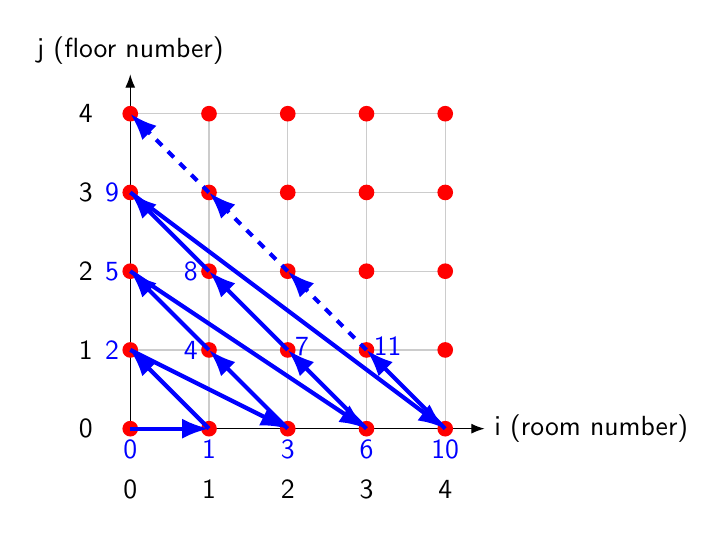
\begin{tikzpicture}[
    >=Latex, 
    node style/.style={circle, fill=red, inner sep=2pt, font=\bfseries\sffamily, text=white},
    label style/.style={font=\sffamily},
    grid style/.style={line width=0.5pt, gray!40},
    path style/.style={line width=1.5pt, blue, ->},
    dashed path style/.style={line width=1.5pt, blue, dashed, ->}
]

% Draw the grid
\draw[grid style] (0,0) grid (4,4);

% Draw the axes and labels
\draw[->] (0,0) -- (4.5,0) node[right, label style] {i (room number)};
\draw[->] (0,0) -- (0,4.5) node[above, label style] {j (floor number)};

% Draw the nodes for the grid points
\foreach \x in {0,1,2,3,4} {
    \foreach \y in {0,1,2,3,4} {
        \node[node style, label={[label style]above right:}] at (\x, \y) {};
    }
}

% Add labels for the axes values
\foreach \i in {0,1,2,3,4} {
    \node[below=15pt, label style] at (\i,0) {\i};
}
\foreach \j in {0,1,2,3,4} {
    \node[left=10pt, label style] at (0,\j) {\j};
}

% Define the path based on the Cantor pairing function
% Path for n=0 to n=10
%\draw[path style] (0,0) -- node[above, pos=0.5, font=\sffamily] {0} (0,0.1);
\draw[path style] (0,0) -- (1,0) node[below, pos=0, font=\sffamily] {0};
\draw[path style] (1,0) -- (0,1) node[below, pos=0, font=\sffamily] {1};
\draw[path style] (0,1) -- (2,0) node[left, pos=0, font=\sffamily] {2};
\draw[path style] (2,0) -- (1,1) node[below, pos=0, font=\sffamily] {3};
\draw[path style] (1,1) -- (0,2) node[left, pos=0, font=\sffamily] {4};
\draw[path style] (0,2) -- (3,0) node[left, pos=0, font=\sffamily] {5};
\draw[path style] (3,0) -- (2,1) node[below, pos=0, font=\sffamily] {6};
\draw[path style] (2,1) -- (1,2) node[right, pos=0.05, font=\sffamily] {7};
\draw[path style] (1,2) -- (0,3) node[left, pos=0, font=\sffamily] {8};
\draw[path style] (0,3) -- (4,0) node[left, pos=0, font=\sffamily] {9};
\draw[path style] (4,0) -- (3,1) node[below, pos=0, font=\sffamily] {10};
\draw[dashed path style] (3,1) -- (2,2) node[right, pos=0.05, font=\sffamily] {11};
\draw[dashed path style] (2,2) -- (1,3);% node[above, pos=0.5, font=\sffamily] {13};
\draw[dashed path style] (1,3) -- (0,4);% node[above, pos=0.5, font=\sffamily] {14};
%\draw[path style] (0,4) -- (4,1) node[above, pos=0.5, font=\sffamily] {15};
%\draw[path style] (4,1) -- (3,2) node[above, pos=0.5, font=\sffamily] {16};
%\draw[path style] (3,2) -- (2,3) node[above, pos=0.5, font=\sffamily] {17};
%\draw[path style] (2,3) -- (1,4) node[above, pos=0.5, font=\sffamily] {18};
%\draw[path style] (1,4) -- (4,2) node[above, pos=0.5, font=\sffamily] {19};
%\draw[path style] (4,2) -- (3,3) node[above, pos=0.5, font=\sffamily] {20};
%\draw[path style] (3,3) -- (2,4) node[above, pos=0.5, font=\sffamily] {21};
%\draw[path style] (2,4) -- (4,3) node[above, pos=0.5, font=\sffamily] {22};
%\draw[path style] (4,3) -- (3,4) node[above, pos=0.5, font=\sffamily] {23};
%\draw[path style] (3,4) -- (4,4) node[above, pos=0.5, font=\sffamily] {24};
\end{tikzpicture}
%\end{document}


\end{center}

%This one-to-one correspondence means that the set of all pairs of rooms and floors is, in fact, the same ``size'' as the set of all natural numbers. It's a concept that's a little hard to wrap your head around, but it's one of the great secrets of infinity!

This one-to-one correspondence means that the set of all pairs of rooms and floors is, in fact, the same ``size'' as the set of all natural numbers. This challenges one of our most basic intuitions. As the mathematician David Hilbert pointed out, when dealing with finite sets, a part is always smaller than the whole. But when we are dealing with infinite sets, this principle no longer applies. As he said: ``Hier gilt nun schon der Satz: ,,Der Teil ist kleiner als das Ganze'' nicht mehr.'' (Hilbert, 1925 in lecture ``\"{U}ber das Unendliche''). It's a concept that's a little hard to wrap your head around, but it's one of the great secrets of infinity!


\clearpage
\includepdf[pages={1},
            pagecommand={\thispagestyle{fancy}}, % Apply your custom 'fancy' style
            fitpaper=true,
            noautoscale
           ]{pigfootball.pdf}
\clearpage
\pagenumbering{gobble}
\thispagestyle{empty}
\includepdf[pages=-]{backcover.en.pdf}

\end{document}
